\chapter{Hyperbolic plane}\label{chap:poincare}

\begin{figure}[!ht]
\vspace*{-9mm}
\centering
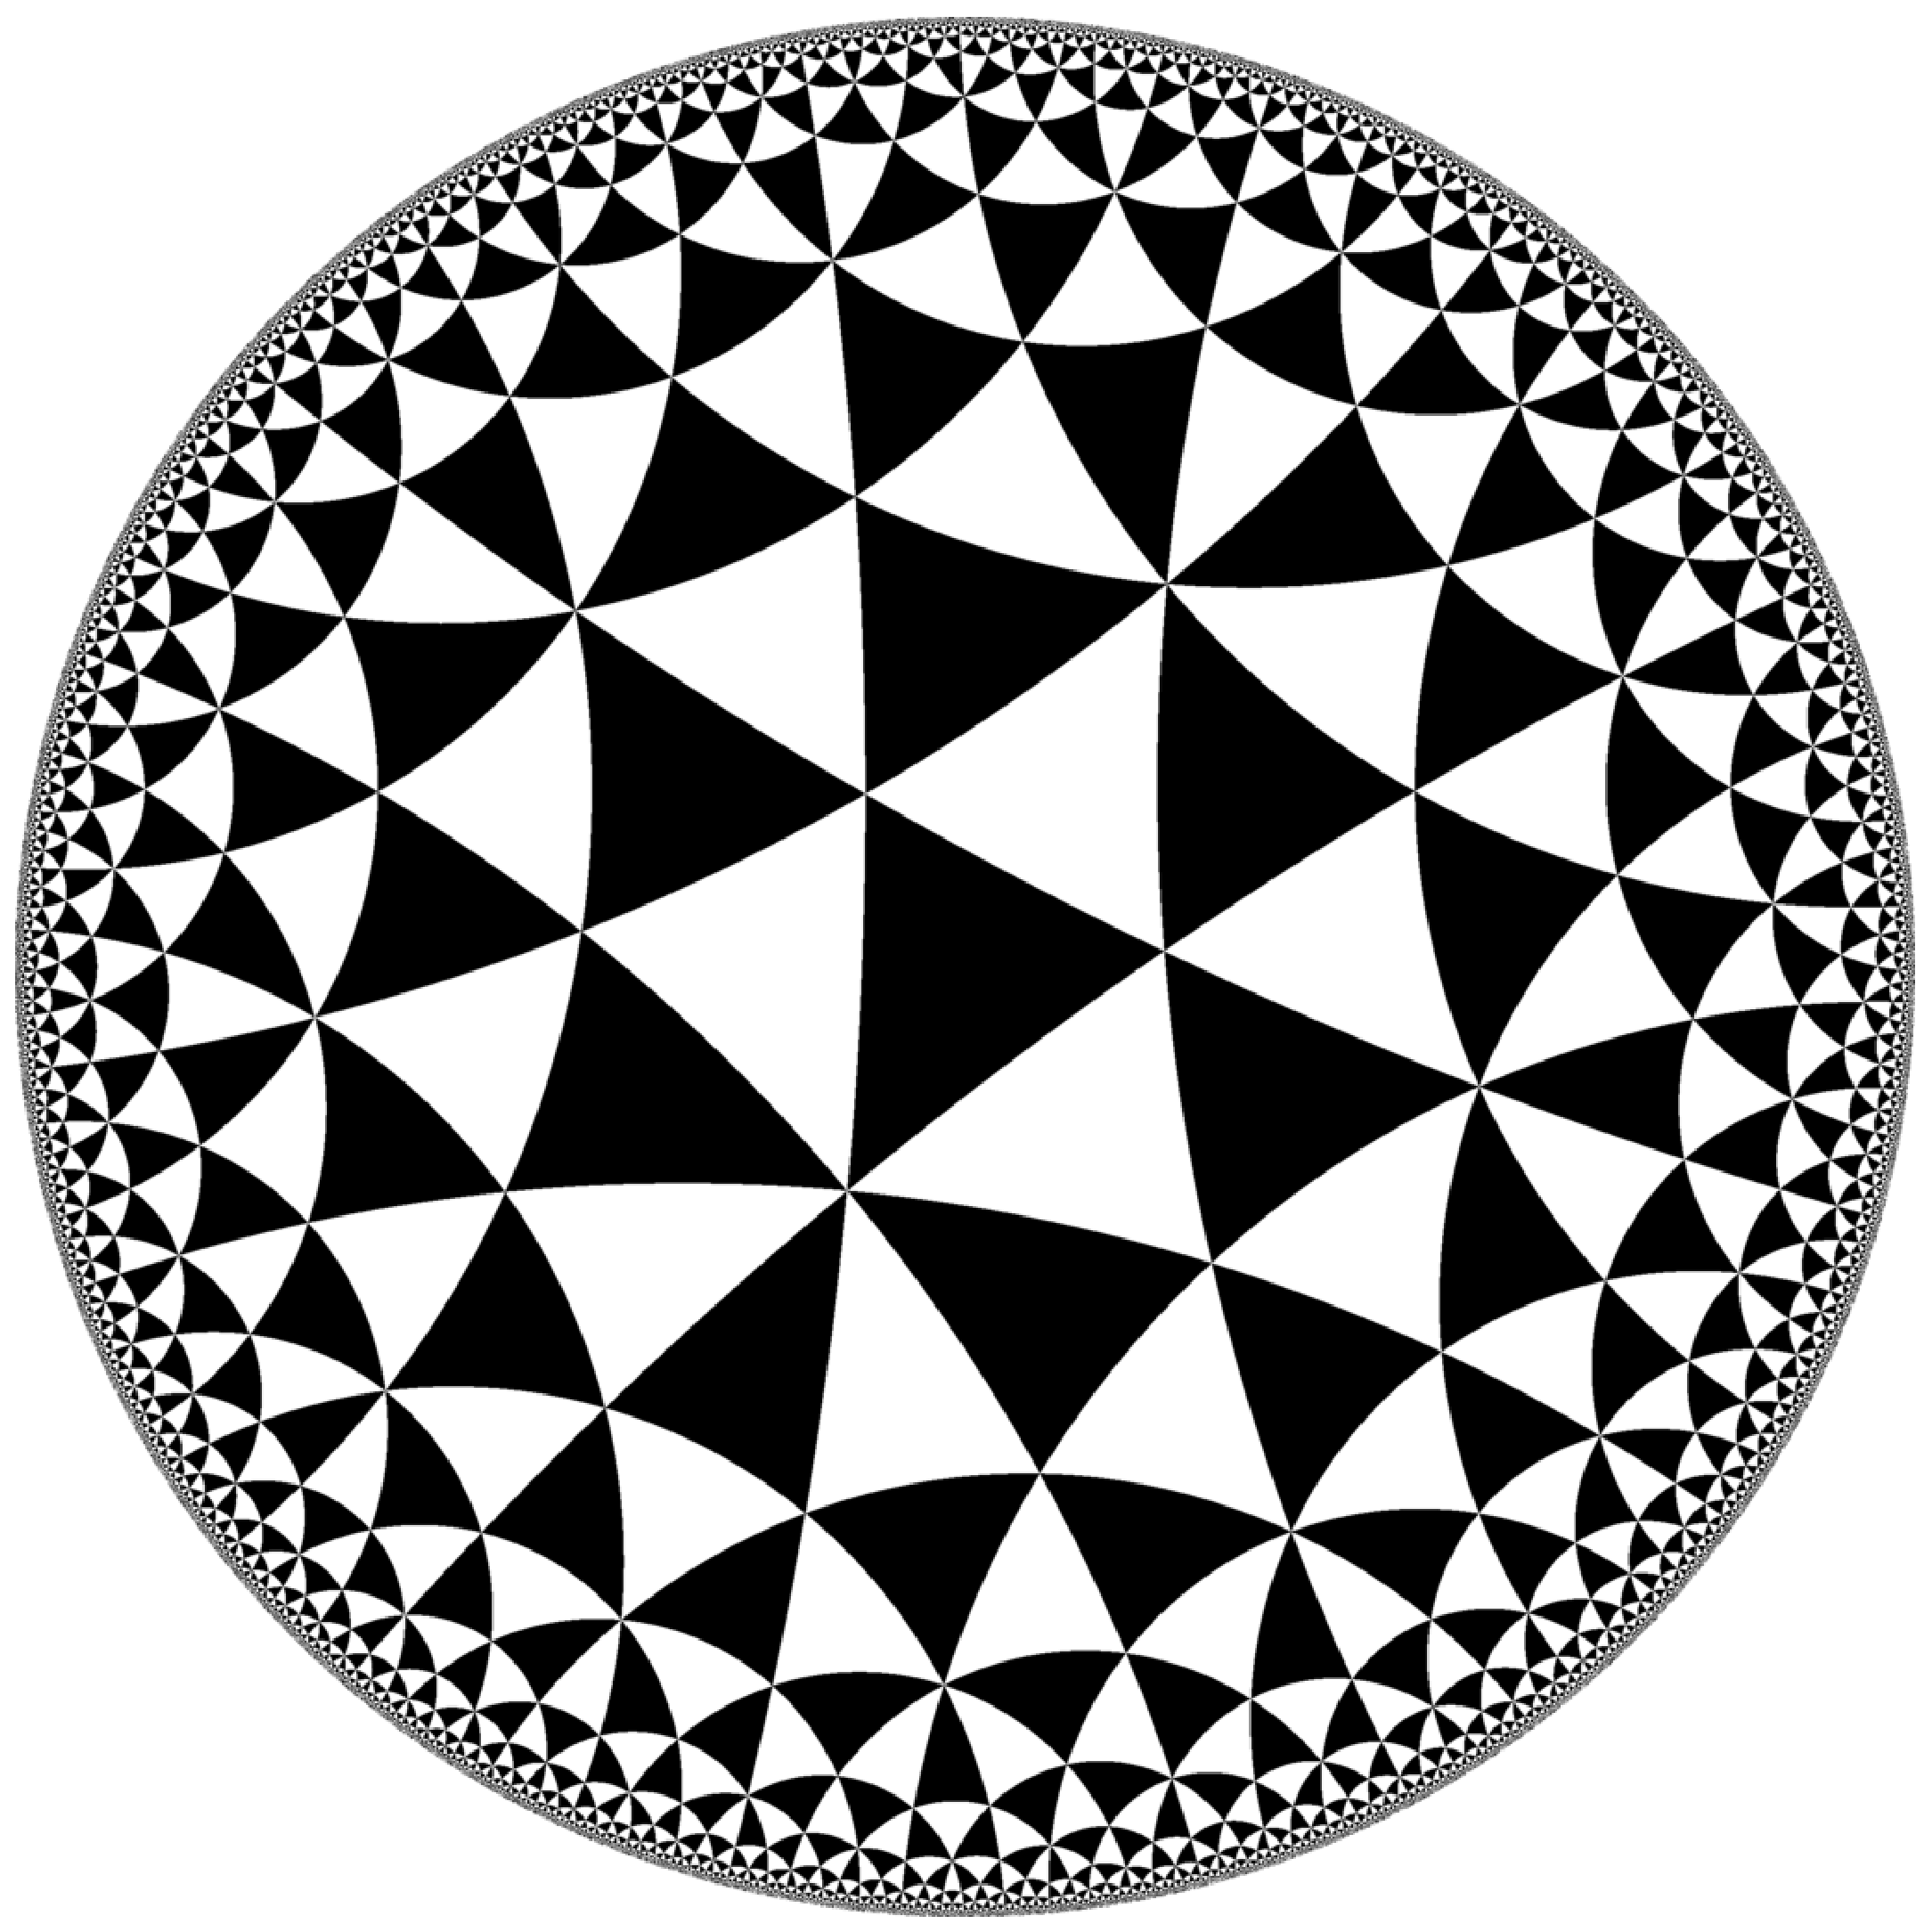
\includegraphics[scale=0.25]{pics/H2checkers_334}
\end{figure}

In this chapter, we use inversive geometry 
to construct a model of a hyperbolic plane --- a neutral plane that is not Euclidean.

Namely, we construct the so-called \index{conformal disc model}\emph{conformal disc model} of the hyperbolic plane.
This model was discovered by Eugenio Beltrami \cite{beltrami},
and it is commonly referred to as the {}\emph{Poincar\'e disc model}. 

The figure above shows the conformal disc model of the hyperbolic plane which is divided into congruent triangles with angles $\tfrac\pi3$, $\tfrac\pi3$, and~$\tfrac\pi4$.

\section{Conformal disc model}
\label{sec:conformal-model}

In this section, we give new names for certain objects in the Euclidean plane
which will represent lines, angle measures, and distances in the hyperbolic plane.

\parbf{Hyperbolic plane.}
Let us fix a circle on the Euclidean plane 
and call it \index{absolute}\emph{absolute}.
The set of points inside the absolute will be referred to as the \index{hyperbolic!plane}\index{plane!hyperbolic plane}\emph{hyperbolic plane} (or \index{plane!h-plane}\index{h-plane}\emph{h-plane}).

The points on the absolute do \textit{not} belong to the h-plane.
The points in the h-plane will be also called \index{h-point}\emph{h-points}.

We will often assume that the absolute is a unit circle.



\parbf{Hyperbolic lines.}
The intersections of the h-plane with circlines that are perpendicular to the absolute are called {}\emph{hyperbolic lines} or \index{h-line}\emph{h-lines}.

\begin{wrapfigure}{o}{48mm}
\centering
\includegraphics{mppics/pic-190}
\end{wrapfigure}

By Corollary~\ref{cor:h-line}, there exists a unique h-line that passes thru any two distinct h-points $P$ and~$Q$.
This h-line will be denoted by~\index{62@$(PQ)_h$, $[PQ)_h$,$[PQ]_h$}$(PQ)_h$.

The arcs of hyperbolic lines will be called {}\emph{hyperbolic segments} or \index{h-segment}\emph{h-segments}.
An h-segment with endpoints $P$ and $Q$ will be denoted as~$[PQ]_h$.

The portion of an h-line on one side of a point will be called a {}\emph{hyperbolic half-line} (or \index{h-half-line}\emph{h-half-line}).
More precisely, an h-half-line is the intersection of the h-plane with an arc that is perpendicular to the absolute and has exactly one of its endpoints in the h-plane.
An h-half-line starting at $P$ and passing thru $Q$ will be denoted as~$[PQ)_h$.

If $\Gamma$ is the circline containing the h-line $(PQ)_h$, then the points ($A$ and $B$ in the picture) where $\Gamma$ intersects the absolute are called
\index{point!ideal point}\index{ideal!point}\emph{ideal points} of~$(PQ)_h$.
(The ideal points of an h-line do not belong to the h-line.)

An ordered triple of h-points, say $(P,Q,R)$, will be called an {}\emph{h-triangle $PQR$} and denoted by \index{21@$\triangle_h$}$\triangle_h P Q R$.

It is important to clarify that at this point, that \textit{so far an h-line $(PQ)_h$ is just a subset of the h-plane},
but soon we will introduce h-distance 
and show that $(PQ)_h$ is a line for the h-distance in the sense of the Definition~\ref{def:line}. 

\begin{thm}{Exercise}\label{ex:ideal-line-unique}
Show that an h-line is uniquely determined by its ideal points.
\end{thm}

\begin{thm}{Exercise}\label{ex:1ideal-line-unique}
Show that an h-line is uniquely determined by one of its ideal points and one h-point on it.
\end{thm}

\begin{thm}{Exercise}\label{ex:line/h-line}
Show that an h-segment $[PQ]_h$ coincides with the Euclidean segment $[PQ]$
if and only if the line $(PQ)$ passes thru the center of the absolute.
\end{thm}

\parbf{Hyperbolic distance.}\label{h-dist}
Consider two distinct h-points $P$ and $Q$,
and let $A$ and $B$ denote the ideal points of $(PQ)_h$.
Without loss of generality, we may assume that on the Euclidean circline containing the h-line $(PQ)_h$, the points $A,P,Q,B$ appear in the same order.

Consider the function 
$$\delta(P,Q)\df\frac{AQ\cdot PB}{AP\cdot QB}.$$
The right-hand side is a cross-ratio;
by Theorem~\ref{lem:inverse-4-angle} it is invariant under inversion.
We set $\delta(P,P)=1$ for any h-point~$P$.
Let us define h-distance as the logarithm of $\delta$; that is,
$$PQ_h\df\ln[\delta(P,Q)].$$

The proof that $PQ_h$ is a metric on the h-plane will be given later.
For now, it is just a function that returns a real value $PQ_h$ for any pair of h-points $P$ and~$Q$.

\begin{thm}{Exercise}\label{ex:h-dist-eq}
Let $O$ be the center of the absolute.
Assume that h-points $O$, $X$, and $Y$ lie on an h-line in the same order, and $OX\z=XY$.
Prove that $OX_h<XY_h$.
\end{thm}


\parbf{Hyperbolic angles.}\label{h-angle measure}
Consider three h-points $P$, $Q$, and $R$
such that $P\ne Q$ and $R\ne Q$.
The \index{hyperbolic!angle}\emph{hyperbolic angle $PQR$} (briefly $\angle_h PQR$)\index{11@$\angle_h$, $\measuredangle_h$} consists of the ordered pair of h-half-lines $[QP)_h$ and $[QR)_h$.

Let $[QX)$ and $[QY)$ be (Euclidean) half-lines 
that are tangent to $[QP]_h$ and $[QR]_h$ 
at~$Q$.
Then the \index{angle!measure!hyperbolic angle measure}\index{hyperbolic!angle measure}\emph{hyperbolic angle measure} (or \index{h-angle measure}\emph{h-angle measure}) of $\angle_h PQR$ is denoted by
$\measuredangle_h PQR$ and is defined as
$\measuredangle XQY$.

\begin{thm}{Exercise}\label{ex:h-perp-unique}
Let $P$ be an h-point that does not lie on an h-line~$\ell$.
Show that there is a unique h-line thru $P$ that is perpendicular to~$\ell$.
\end{thm}

\section{Plan of the proof}

We have introduced all the {}\emph{h-notions} needed in the formulation of the axioms \ref{def:birkhoff-axioms:0}--\ref{def:birkhoff-axioms:3} and h-\ref{def:birkhoff-axioms:4}.
It remains to show that all these axioms hold; 
this will be done by the end of this chapter.

Once our proofs are complete, we will have a model that serves as an example of a neutral plane.
After that we can use axiomatic approach in the h-plane;
for example, Exercise~\ref{ex:h-perp-unique} can be proved the same way as Theorem~\ref{perp:ex+un}.

Most importantly we will prove the ``if''-part of Theorem~\ref{thm:consistent}.

Indeed, any statement in hyperbolic geometry can be restated in the Euclidean plane using the introduced h-notions.
Consequently, if the system of axioms \ref{def:birkhoff-axioms:0}--\ref{def:birkhoff-axioms:3}, and h-\ref{def:birkhoff-axioms:4} leads to a contradiction, then so does the system axioms \ref{def:birkhoff-axioms:0}--\ref{def:birkhoff-axioms:4}.

\section{Auxiliary statements}

One may compare the conformal model with a telescope --- it makes it possible to see the h-plane from the Euclidean plane.
Continuing this analogy further, we may say that the following lemma will be used to \textit{aim} the telescope at any particular point in the h-plane.

\begin{thm}{Lemma}\label{lem:P-->O} 
Consider an h-plane with a unit circle $\Omega$ as the absolute.
Let $O$ be the center of $\Omega$ and $P$ be another h-point.
Then there is a circle $\Gamma$ perpendicular to the absolute such that $O$ is the inverse of $P$ across~$\Gamma$.

Moreover, $\Gamma$ has radius $\tfrac{\sqrt{1-OP^2}}{OP}$,
and its center $P'$ is the inverse of $P$ across the absolute. 
\end{thm}

\begin{wrapfigure}[8]{o}{45mm}
\vskip-6mm
\centering
\includegraphics{mppics/pic-192}
\end{wrapfigure}

\parit{Proof.}
Let $P'$ be the inversion of $P$ across the absolute.
Choose a point $T$ on the absolute such that $\angle OPT$ is right.
Let $\Gamma$ be the circle thru $T$ with center $P'$.

By \ref{lem:inversion-sim}, $\triangle OPT\sim \triangle OTP'$.
It follows that $\angle OTP'$ is right and $\Gamma\perp\Omega$.

By AA, $\triangle TPP'\sim \triangle OTP'$
(the angle at $P'$ is shared, and $\angle TPP'$ and $\angle OTP'$ are right). 
Therefore $\tfrac{OP'}{P'T}=\tfrac{P'T}{PP'}$; so, $O$ is the inversion of $P$ across~$\Gamma$.

Note that $OP'\cdot OP=OT^2$.
By the Pythagorean theorem $P'T^2\z=P'P^2+PT^2$ and $PT^2=OT^2-PO^2$.
Since $P'P=OP'-OP$ and $OT=1$, we get $P'T=\tfrac{\sqrt{1-OP^2}}{OP}$,
and the second statement follows.
\qeds

Assume $\Gamma$ is a circline that is perpendicular to the absolute.
Consider the inversion $X\mapsto X'$ across $\Gamma$;
if $\Gamma$ is a line, set $X\mapsto X'$ to be the reflection across~$\Gamma$.

The following observation says that the map $X\mapsto X'$ respects all the notions introduced in the previous section.
Together with the lemma above, it implies that in any problem that is formulated entirely \textit{in h-terms} we can assume that a given h-point lies in the center of the absolute.

\begin{thm}{Main observation}\label{thm:main-observ}
The map $X\mapsto X'$ described above is a bijection from the h-plane to itself. 
Moreover, for any h-points $P$, $Q$, $R$ such that $P\ne Q$ and $Q\ne R$, the following conditions hold:
\begin{enumerate}[(a)]
\item\label{h-line-to-hline} The h-line $(PQ)_h$, h-half-line $[PQ)_h$, and h-segment $[PQ]_h$ are transformed into $(P'Q')_h$, $[P'Q')_h$, and $[P'Q']_h$ respectively.
\item\label{h-reflect} $\delta(P',Q')=\delta(P,Q)$ and $P'Q'_h=PQ_h$.
\item\label{h-angle-mes} 
$\measuredangle_h P'Q'R'\equiv-\measuredangle_h PQR$.
\end{enumerate}

\end{thm}

It is instructive to compare this observation with Proposition~\ref{prop:reflection}.

\parit{Proof.}
According to Theorem~\ref{thm:perp-inverse}, the map sends the absolute to itself. 
Therefore the points on $\Gamma$ do not move.
It follows that points inside of the absolute remain inside after the mapping.
Whence the $X\mapsto X'$ is a bijection from the h-plane to itself.


Part~\textit{(\ref{h-line-to-hline})} follows from \ref{thm:inverse-cline} and \ref{thm:angle-inversion}.

Part~\textit{(\ref{h-reflect})} follows from Theorem~\ref{lem:inverse-4-angle}.

Part~\textit{(\ref{h-angle-mes})} follows from Theorem~\ref{thm:angle-inversion}.
\qeds


\begin{thm}{Lemma}\label{lem:O-h-dist}
Assume that the absolute is a unit circle centered at~$O$.
Given an h-point $P$, set $x=OP$ and $y=OP_h$.
Then
\begin{align*}
y&=\ln\frac{1+x}{1-x}
&
&\text{and}
&
x&=\frac{e^y-1}{e^y+1}.
\end{align*}
 
\end{thm}

Observe that according to the lemma, $OP_h\to \infty$ as $OP\to 1$.
That is, if $P$ the approaches absolute in the Euclidean sense, it escapes to infinity in the h-sense.

\begin{wrapfigure}[6]{o}{38mm}
\vskip-4mm
\centering
\includegraphics{mppics/pic-194}
\end{wrapfigure}

\parit{Proof.}
The h-line $(OP)_h$ lies on a diameter of the absolute.
If $A$ and $B$ are the ideal points as in the definition of the h-distance, then
\begin{align*}
OA&=OB=1,
\\ 
PA&=1+x,
\\
PB&=1-x.\end{align*}
In particular,
\begin{align*}
y&=\ln \frac{AP\cdot BO}{PB\cdot OA}=\ln\frac{1+x}{1-x}.
\end{align*}

Taking the exponential function of the left and the right-hand side and applying obvious algebra manipulations, we get that
$$x=\frac{e^y-1}{e^y+1}.$$
\qedsf


\begin{thm}{Lemma}\label{lem:h-tiangle=}
Assume that points $P$, $Q$, and $R$ appear on an h-line in the same order.
Then 
$$PQ_h+QR_h=PR_h.$$ 

\end{thm}

\parit{Proof.}
Note that
$$PQ_h+QR_h=PR_h$$
is equivalent to 
\[\delta(P,Q)\cdot\delta(Q,R)=\delta(P,R).\eqlbl{eq:deltaPQR}\]

Let $A$ and $B$ be the ideal points of~$(PQ)_h$. 
Without loss of generality, we can assume that the points $A$, $P$, $Q$, $R$, and $B$ appear in the same order on the circline containing $(PQ)_h$.
Then
\begin{align*}
\delta(P,Q)\cdot\delta(Q,R)
&=
\frac{AQ\cdot BP}{QB\cdot PA}\cdot\frac{AR\cdot BQ}{RB\cdot QA}=
\\
&=\frac{AR\cdot BP}{RB\cdot PA}=
\\
&=\delta(P,R).
\end{align*}
Hence \ref{eq:deltaPQR} follows.
\qeds

Let $P$ be an h-point and $\rho>0$.
The set of all h-points $Q$ such that $PQ_h=\rho$ is called an \index{h-circle}\emph{h-circle} with the center $P$ and the \index{h-radius}\emph{h-radius} $\rho$.

\begin{thm}{Lemma}\label{lem:h-circle=circle}
Any h-circle is a Euclidean circle that lies completely in the h-plane.

More precisely for any h-point $P$ and $\rho\ge 0$
there is a $\hat\rho\ge 0$ and a point $\hat P$ such that 
$$PQ_h= \rho
\quad 
\iff
\quad
\hat PQ= \hat\rho$$
for any h-point~$Q$.

Moreover, if $O$ is the center of the absolute, then 
\begin{enumerate}
\item $\hat O=O$ for any $\rho$ and
\item $\hat P\in (OP)$ for any $P\ne O$.
\end{enumerate}

\end{thm}

\begin{wrapfigure}{o}{33mm}
\vskip-4mm
\centering
\includegraphics{mppics/pic-196}
\end{wrapfigure}

\parit{Proof.}
According to Lemma~\ref{lem:O-h-dist}, 
$OQ_h\z= \rho$ if and only if $$OQ= \hat\rho=\frac{e^\rho-1}{e^\rho+1}.$$
Therefore, the locus of h-points $Q$ such that $OQ_h= \rho$ is a Euclidean circle, 
denote it by $\Delta_\rho$.

If $P\ne O$, then by Lemma~\ref{lem:P-->O} and the main observation (\ref{thm:main-observ})
there is an inversion that respects all h-notions and sends $O\mapsto P$.

Let $\Delta_\rho'$ be the inverse of $\Delta_\rho$.
Since the inversion preserves the h-distance,
$PQ_h=\rho$ if and only if $Q\z\in\Delta_\rho'$.

According to Theorem~\ref{thm:inverse-cline}, $\Delta_\rho'$ is a Euclidean circle.
Let $\hat P$ and $\hat\rho$ denote the Euclidean center and radius of $\Delta_\rho'$.

Finally, note that $\Delta_\rho'$ reflects to itself across $(OP)$;
that is, the center $\hat P$ lies on~$(OP)$.
\qeds

\begin{thm}{Exercise}\label{ex:h-circle=circle}
Describe a nondegenerate h-triangle $\triangle_hPQR$ that does not have an h-circumcircle;
that is, its vertices $P$, $Q$, and $R$ do not lie on an h-circle or h-line.
\end{thm}

\section[Axioms]{Axioms}
\subsection*{Axiom~\ref{def:birkhoff-axioms:0}}

Evidently, the h-plane contains at least two points.
Therefore, to show that Axiom~\ref{def:birkhoff-axioms:0} holds in the h-plane, we need to show that the h-distance defined in Section~\ref{sec:conformal-model} is a metric;
that is, the conditions \textit{(\ref{def:metric-space:a})}--\textit{(\ref{def:metric-space:d})} 
in Definition~\ref{def:metric-space} hold for the h-distance.


The following claim says that the h-distance satisfies conditions \textit{(\ref{def:metric-space:a})} 
and \textit{(\ref{def:metric-space:b})}.

\begin{thm}{Claim}
For any pair of h-points $P$ and $Q$, we have
$PQ_h\ge 0$
and $PQ_h=0$ if and only if $P=Q$.
\end{thm}


\parit{Proof.}
According to Lemma~\ref{lem:P-->O}
and the main observation (\ref{thm:main-observ}), 
we can assume that $Q$ is the center of the absolute.
In this case
$$
\delta(Q,P)=\frac{1+QP}{1-QP}\ge 1$$
and therefore
$$QP_h=\ln[\delta(Q,P)]\ge 0.$$
Moreover, the equalities hold if and only if $P=Q$.
\qeds

The following claim says that the h-distance meets~\ref{def:metric-space}\textit{\ref{def:metric-space:c}}.

\begin{thm}{Claim}
For any h-points $P$ and $Q$, we have
$PQ_h=QP_h$.
\end{thm}

\parit{Proof.}
Let $A$ and $B$ be ideal points of $(PQ)_h$ and
$A,P,Q,B$ appear on the circline containing $(PQ)_h$ in the same order.

{

\begin{wrapfigure}{o}{33mm}
\vskip-5mm
\centering
\includegraphics{mppics/pic-198}
\end{wrapfigure}

Then
\begin{align*}
PQ_h
&=\ln\frac{AQ\cdot BP}{QB\cdot PA}
=
\\
&=\ln\frac{BP\cdot AQ}{PA\cdot QB}=
\\
&=QP_h.
\end{align*}
\qedsf

}

The following claim shows, in particular, that
the triangle inequality 
(which is condition \ref{def:metric-space}\textit{\ref{def:metric-space:d}})
holds for $h$-distance.

\begin{thm}{Claim}\label{clm:h-dist+trig-inq}
Given a triple of h-points $P$, $Q$, and $R$,
we have
\[PQ_h+QR_h\ge PR_h.\]
Moreover, the equality holds if and only if $P$, $Q$, and $R$ lie on one h-line in the same order.
\end{thm}

\parit{Proof.}
Without loss of generality, we may assume that $P$ is the center of the absolute
and 
$0<QR_h\le PQ_h$.

Let $\Delta$ be the h-circle with the center $Q$ and h-radius $QR_h$.
Choose points $S$ and $T$ on the intersection of $(PQ)$ with~$\Delta$ so that $P$, $S$, $Q$, and $T$ appear on the h-line in the same order.
The latter is possible by Lemma~\ref{lem:h-tiangle=}, since $QS_h\z=QT_h\z=QR_h\z\le PQ_h$.

{

\begin{wrapfigure}{o}{35mm}
\vskip-0mm
\centering
\includegraphics{mppics/pic-200}
\end{wrapfigure}

According to Lemma~\ref{lem:h-circle=circle}, $\Delta$ is a Euclidean circle;
let $\hat Q$ be its Euclidean center.

Note that $\hat QS\z=\hat QT\z=\hat QR$.
By the Euclidean triangle inequality,
$$PT
=
P\hat Q+\hat Q R
\ge 
PR,
\eqlbl{RT>RQ}$$
and the equality holds if and only if $T=R$. 

By Lemma~\ref{lem:O-h-dist},
\begin{align*}
PT_h&=\ln\frac{1+PT}{1-PT},\\
PR_h&=\ln\frac{1+PR}{1-PR}.
\end{align*}
Note that the function $x\mapsto\ln\frac{1+x}{1-x}$ is increasing for $0\le x<1$.
Therefore, \ref{RT>RQ} implies
$$PT_h\ge PR_h;$$
moreover, the equality holds if and only if $T\z=R$.

}

Finally, applying Lemma~\ref{lem:h-tiangle=} again, 
we get that
$$PT_h=PQ_h+QR_h.$$
Hence the claim follows.
\qeds

\subsection*{Axiom~\ref{def:birkhoff-axioms:1}}

Once the following claim is proved,
Axiom~\ref{def:birkhoff-axioms:1} 
follows from Corollary~\ref{cor:h-line}.

\begin{thm}{Claim}
A subset of the h-plane is an h-line if and only if it forms a line for the h-distance in the sense of Definition~\ref{def:line}.
\end{thm}

\parit{Proof.}
Let $\ell$ be an h-line.
Applying the main observation (\ref{thm:main-observ}) we can assume that $\ell$ contains the center of the absolute.
In this case, $\ell$ is an intersection of a diameter of the absolute and the h-plane.
Let $A$ and $B$ be the endpoints of the diameter.

\begin{wrapfigure}{o}{29mm}
\vskip-3mm
\centering
\includegraphics{mppics/pic-201}
\vskip-2mm
\end{wrapfigure}

Consider the map $\iota\:\ell\to \mathbb{R}$ defined as
$$\iota(X)=\ln \frac{AX}{XB}.$$
Note that $\iota\:\ell\to \mathbb{R}$ is a bijection.

Furthermore, if $X,Y\in \ell$ and the points $A$, $X$, $Y$, and $B$ appear on $[AB]$ in the same order, then
\[\iota(Y)-\iota(X)=\ln \frac{AY}{YB}-\ln \frac{AX}{XB}=\ln \frac{AY\cdot BX}{YB\cdot XB}=XY_h.\]

We have shown that any h-line is a line for h-distance.
The converse follows from Claim~\ref{clm:h-dist+trig-inq}.
\qeds


\subsection*{Axiom~\ref{def:birkhoff-axioms:2}}

The first part of Axiom~\ref{def:birkhoff-axioms:2} follows directly from the definition of the h-angle measure (defined in Section~\ref{sec:conformal-model}).
It remains to show that $\measuredangle_h$ satisfies the conditions \ref{def:birkhoff-axioms:2a}, \ref{def:birkhoff-axioms:2b}, and \ref{def:birkhoff-axioms:2c} (see Section~\ref{sec:axioms}).

The following two claims say that
$\measuredangle_h$ satisfies
 \ref{def:birkhoff-axioms:2a} and \ref{def:birkhoff-axioms:2b}.

\begin{thm}{Claim}\label{clm:h2a}
Given an h-half-line $[O P)_h$ and $\alpha\in(-\pi,\pi]$, there is a unique h-half-line $[O Q)_h$ such that $\measuredangle_h P O Q= \alpha$.
\end{thm}

\begin{thm}{Claim}\label{clm:h2b}
For any h-points $P$, $Q$, and $R$ distinct from an h-point $O$, we have
$$\measuredangle_h P O Q+\measuredangle_h Q O R
\equiv\measuredangle_h P O R.$$

\end{thm}

\parit{Proof of \ref{clm:h2a} and \ref{clm:h2b}.}
Applying the main observation, 
we may assume that $O$ is the center of the absolute.
In this case, for any h-point $P\z\ne O$, the h-half-line
$[OP)_h$ is the intersection of the Euclidean half-line $[OP)$ with the h-plane.
Hence \ref{clm:h2a} and \ref{clm:h2b} 
follow from the axioms \ref{def:birkhoff-axioms:2a} and \ref{def:birkhoff-axioms:2b} of the Euclidean plane.
\qeds

The following claim says that
$\measuredangle_h$ satisfies
 \ref{def:birkhoff-axioms:2c}.

\begin{thm}{Claim}\label{clm:h2c}
The function 
$$\measuredangle_h\:(P,Q,R)\mapsto\measuredangle_h P Q R$$
is continuous at any triple of points $(P,Q,R)$
such that $Q\ne P$, $Q\ne R$, and $\measuredangle_h P Q R\ne\pi$.
\end{thm}

\parit{Proof.}
Suppose that $O$ denotes the center of the absolute.
We can assume that $Q$ is distinct from~$O$;
the latter follows from the main observation.

\begin{wrapfigure}{o}{45mm}
\vskip-4mm
\centering
\includegraphics{mppics/pic-199}
\end{wrapfigure}

Let $Z$ be the inverse of $Q$ across the absolute;
denote by $\Gamma$ the circle with the center at~$Z$ that is perpendicular to the absolute.
According to Lemma~\ref{lem:P-->O},
point $O$ is the inverse of $Q$ across~$\Gamma$.

Let $P'$ and $R'$ be the inversions across $\Gamma$ of the points $P$ and $R$ respectively.
The point $P'$ is completely determined by $Q$ and $P$.
Moreover, the map $(Q,P)\mapsto P'$ is continuous at any pair of h-points $(Q,P)$ such that $Q\ne O$.
The same is true for the map $(Q,R)\mapsto R'$.

According to the main observation 
$$\measuredangle_h P Q R\equiv -\measuredangle_h P' O R'.$$
Since $\measuredangle_h P' O R'=\measuredangle P' O R'$ and 
the maps $(Q,P)\mapsto P'$, $(Q,R)\mapsto R'$ are continuous,
the claim follows from the corresponding axiom of the Euclidean plane.
\qeds

\subsection*{Axiom~\ref{def:birkhoff-axioms:3}}

The following claim says that Axiom~\ref{def:birkhoff-axioms:3} holds in the h-plane.

\begin{thm}{Claim}
In the h-plane, we have
$\triangle_h P Q R 
\cong
\triangle_h P' Q' R'$
if and only if 
\begin{align*}
Q' P'_h&=Q P_h, & Q' R'_h&= Q R_h &&\text{and}
&\measuredangle_h P' Q' R'&=\pm\measuredangle P Q R.
\end{align*}
 
\end{thm}

\parit{Proof.}
Applying the main observation, 
we can assume that $Q$ and $Q'$ coincide with the center of the absolute; in particular, $Q=Q'$.
In this case, 
$$\measuredangle P' Q R'=\measuredangle_h P' Q R'=\pm\measuredangle_h P Q R=\pm\measuredangle P Q R.$$
Since 
$$Q P_h=Q P'_h\quad \text{and}\quad Q R_h=Q R'_h,$$
Lemma~\ref{lem:O-h-dist} implies that the same holds for the Euclidean distances;
that is,
$$Q P=Q P'
\quad
\text{and}
\quad
Q R=Q R'.$$
By SAS,
there is a motion of the Euclidean plane that sends
$Q$ to itself,
$P$ to $P'$, 
and $R$ to $R'$.

Note that the center of the absolute is fixed by the corresponding motion.
It follows that this motion gives also a motion of the h-plane;
in particular, the h-triangles 
$\triangle_h P Q R$ and $\triangle_h P' Q R'$ are h-congruent.
\qeds

\subsection*{Axiom h-$\!$\ref{def:birkhoff-axioms:4}}

Finally, we need to check that Axiom~h-$\!$\ref{def:birkhoff-axioms:4} in Section~\ref{sec:unprovable} holds;
that is, we need to prove the following claim.

{

\begin{wrapfigure}{r}{31mm}
\vskip-4mm
\centering
\includegraphics{mppics/pic-202}
\end{wrapfigure}

\begin{thm}{Claim}
For any h-line $\ell$ and any h-point $P\notin\ell$ there are at least two h-lines that pass thru $P$ 
and have no points of intersection with~$\ell$.
\end{thm}

\parit{Instead of proof.}
Applying the main observation we can assume that $P$ is the center of the absolute.

The remaining part of the proof can be guessed from the picture.
\qeds

}

\begin{thm}{Exercise}\label{ex:3-h-lines}
\begin{enumerate}[(a)]
\item Show that in the h-plane there are three mutually parallel h-lines 
such that any pair of these three lines lies on one side of the remaining h-line.
\item Draw three h-lines $\ell$, $m$, and $n$ such that $\ell\parallel m$, $m\parallel n$, but $\ell\nparallel n$.
Conclude that the parallelness is not an equivalence relation for h-lines.
\end{enumerate}
\end{thm}
 
\section{Hyperbolic trigonometry}
\label{sec:hyp-trig}


This section provides formulas for h-distance using \index{hyperbolic!functions}\emph{hyperbolic functions}.
One of these formulas will be used in the proof of the hyperbolic Pythagorean theorem (\ref{thm:pyth-h-poincare}).

Recall that $\cosh$, $\sinh$, and $\tanh$ denote \index{ch@$\cosh$}\index{hyperbolic!cosine}\emph{hyperbolic cosine}, \index{sh@$\sinh$}\index{hyperbolic!sine}\emph{hyperbolic sine}, and \index{th@$\tanh$}\index{hyperbolic!tangent}\emph{hyperbolic tangent}\label{hyperbolic tangent};
that is, the functions defined by
\[\cosh x\df \tfrac{e^x+e^{-x}}2,
 \quad
 \sinh x\df \tfrac{e^x-e^{-x}}2,
\]
\[\tanh x\df \tfrac{\sinh x}{\cosh x}.
\]

These hyperbolic functions are analogous to sine, cosine, and tangent. 

\begin{thm}{Exercise}\label{ex:hyp-fun}
Prove the following identities:
\[\cosh' x=\sinh x;\quad \sinh'x=\cosh x;\quad (\cosh x)^2-(\sinh x)^2=1.\]
\end{thm}

\begin{thm}{Exercise}\label{ex:O-h-dist}
Assume that the absolute is a unit circle centered at~$O$.
Show that 
\[OP=\tanh(\tfrac12 \cdot OP_h).\]
for any h-point $P$.
\end{thm}

\begin{thm}{Double-argument identities}\label{double-argument}
The identities
\begin{align*}
\cosh (2\cdot x)&=(\cosh x)^2+(\sinh x)^2 
&&\text{and}&
\sinh (2\cdot x)&=2\cdot\sinh x\cdot \cosh x
\end{align*}
hold for any real value $x$.
\end{thm}

\parit{Proof.}
\begin{align*}
(\sinh x)^2+(\cosh x)^2
&=(\tfrac{e^x-e^{-x}}2)^2+(\tfrac{e^x+e^{-x}}2)^2=
\\
&=\tfrac{e^{2\cdot x}+e^{-2\cdot x}}2=
\\
&=\cosh (2\cdot x);
\\
2\cdot\sinh x\cdot \cosh x
&=2\cdot(\tfrac{e^x-e^{-x}}2)\cdot(\tfrac{e^x+e^{-x}}2)=
\\
&=\tfrac{e^{2\cdot x}-e^{-2\cdot x}}2=
\\
&=\sinh (2\cdot x).
\end{align*}
\qedsf

\begin{thm}{Advanced exercise}\label{ex:cosh}
Let $P$ and $Q$ be two h-points distinct from the center of the absolute.
Denote by $P'$ and $Q'$ the inverses of $P$ and $Q$ across the absolute.

\begin{wrapfigure}[20]{r}{40mm}
\centering
\includegraphics{mppics/pic-204}
\end{wrapfigure}

Show that 
\medskip
\begin{enumerate}[(a)]
\item\label{ex:cosh/2} 
$\displaystyle{\cosh[\tfrac12\cdot PQ_h]=\sqrt{\frac{PQ'\cdot P'Q}{PP'\cdot QQ'}};}$
\medskip
\item\label{ex:coshsinh} 
$\displaystyle{\sinh[\tfrac12\cdot PQ_h]=\sqrt{\frac{PQ\cdot P'Q'}{PP'\cdot QQ'}};}$
\medskip
\item\label{ex:coshtanh} 
$\displaystyle{\tanh[\tfrac12\cdot PQ_h]=\sqrt{\frac{PQ\cdot P'Q'}{PQ'\cdot P'Q}};}$
\medskip
\item\label{ex:coshcosh} 
$\displaystyle{\cosh PQ_h=\frac{PQ\cdot P'Q'+PQ'\cdot P'Q}{PP'\cdot QQ'}.}$
\end{enumerate}

\end{thm}
